\begin{figure}
	\centering
	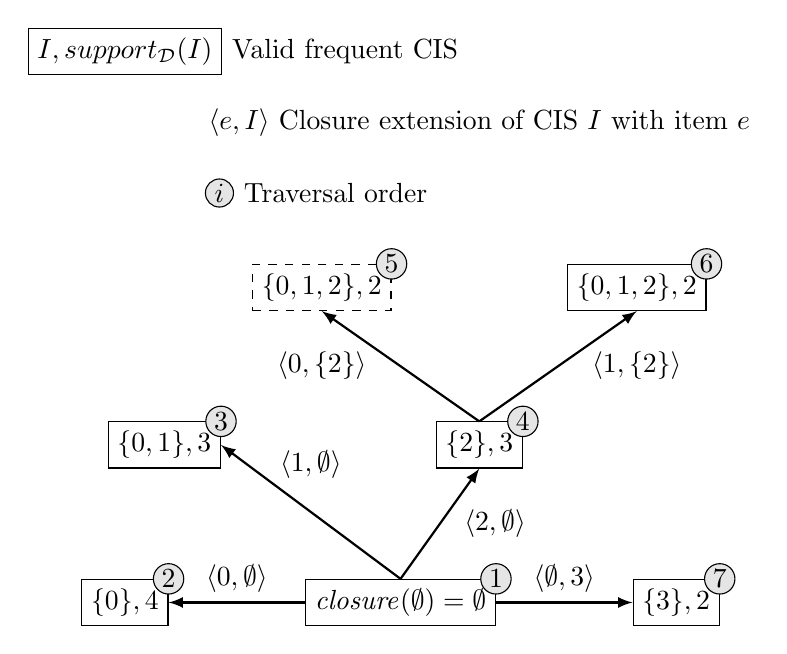
\begin{tikzpicture}[>=latex]
		\node (legenP)[draw,rectangle,minimum width = .8cm,minimum height=.5cm] at (-3.5,7) {$I,support_{\cal D}(I)$};
		\node [right] at (legenP.east) {Valid frequent CIS};

		\node (legenE) at (1, 6.1) {$\langle e,I\rangle$  Closure extension of CIS $I$ with item $e$};

		\node (legenC)[draw,circle,fill=gray!20,inner sep=1pt] at (-2.3,5.2) {$i$};
		\node [right] at (legenC.east) {Traversal order};

		\node (empty) [draw,rectangle,minimum width = .8cm,minimum height=.5cm] at (0,0) {$\mathit{closure}(\emptyset)=\emptyset$};
		\node (step0) [draw,circle,fill=gray!20,inner sep=1pt] at (empty.north east) {1};
		\node (0)     [draw,rectangle,minimum width = .8cm,minimum height=.5cm] at (-3.5,0) {$\{0\},4$};
		\node (step1) [draw,circle,fill=gray!20,inner sep=1pt] at (0.north east) {2};
		\node (1)     [draw,rectangle,minimum width = .8cm,minimum height=.5cm] at (-3,2) {$\{0,1\},3$};
		\node (step2) [draw,circle,fill=gray!20,inner sep=1pt] at (1.north east) {3};
		\node (2)     [draw,rectangle,minimum width = .8cm,minimum height=.5cm] at (1,2) {$\{2\},3$};
		\node (step3) [draw,circle,fill=gray!20,inner sep=1pt] at (2.north east) {4};
		\node (killed)[draw,rectangle,dashed,minimum width = .8cm,minimum height=.5cm] at (-1,4) {$\{0,1,2\},2$};
		\node (step4) [draw,circle,fill=gray!20,inner sep=1pt] at (killed.north east) {5};
		\node (012)   [draw,rectangle,minimum width = .8cm,minimum height=.5cm] at (3,4) {$\{0,1,2\},2	$};
		\node (step5) [draw,circle,fill=gray!20,inner sep=1pt] at (012.north east) {6};
		\node (3)     [draw,rectangle,minimum width = .8cm,minimum height=.5cm] at (3.5,0) {$\{3\},2$};
		\node (step6) [draw,circle,fill=gray!20,inner sep=1pt] at (3.north east) {7};
		\draw [->,thick] (empty.west) -- (0.east) node[above, midway] {$\langle 0, \emptyset\rangle$};
		\draw [->,thick] (empty.north) --(1.east) node[above, midway, yshift=0.3cm] {$\langle 1, \emptyset\rangle$};
		\draw [->,thick] (empty.north)--(2.south) node[above, midway, xshift=0.7cm, yshift=-0.3cm] {$\langle 2, \emptyset\rangle$};
		\draw [->,thick] (empty.east)--(3.west) node[above, midway] {$\langle\emptyset, 3\rangle$};
		\draw [->,thick] (2.north)--(killed.south) node[above, midway, xshift=-1cm, yshift=-0.3cm] {$\langle 0, \{2\}\rangle$};
		\draw [->,thick] (2.north)--(012.south) node[above, midway, xshift=1cm, yshift=-0.3cm] {$\langle 1, \{2\}\rangle$};
	\end{tikzpicture}
	\caption{\label{fig:lcm}
		Frequent CIS enumeration tree on our example dataset (Table~\ref{tab:db}), with $\varepsilon = 2$.
			$\langle e,I\rangle$ denotes the closure extension operation.
		}
\end{figure}
